\documentclass[8pt,aspectratio=169]{beamer}
\usetheme{Madrid}

% Nature Professional Color Palette Definition
\definecolor{ForestGreen}{HTML}{14532D}     % Primary - Deep Forest Green
\definecolor{Teal}{HTML}{0D9488}            % Secondary - Natural Teal
\definecolor{Amber}{HTML}{F59E0B}           % Accent - Warm Amber
\definecolor{Slate}{HTML}{475569}           % Support - Slate Gray
\definecolor{MintCream}{HTML}{F0FDF4}       % Background - Mint Cream
\definecolor{LightGreen}{HTML}{86EFAC}      % Light Green
\definecolor{DarkTeal}{HTML}{0F766E}        % Dark Teal
\definecolor{LightAmber}{HTML}{FCD34D}      % Light Amber

% Apply Nature Professional theme to Beamer
\setbeamercolor{structure}{fg=ForestGreen}
\setbeamercolor{title}{fg=ForestGreen,bg=MintCream}
\setbeamercolor{subtitle}{fg=Teal}
\setbeamercolor{frametitle}{bg=LightGreen!30,fg=ForestGreen}
\setbeamercolor{framesubtitle}{fg=DarkTeal}
\setbeamercolor{normal text}{fg=ForestGreen,bg=white}
\setbeamercolor{background canvas}{bg=MintCream}

% Blocks with nature theme
\setbeamercolor{block title}{bg=Teal,fg=white}
\setbeamercolor{block body}{bg=MintCream,fg=ForestGreen}
\setbeamercolor{block title alerted}{bg=Amber,fg=white}
\setbeamercolor{block body alerted}{bg=LightAmber!20,fg=ForestGreen}
\setbeamercolor{block title example}{bg=ForestGreen,fg=white}
\setbeamercolor{block body example}{bg=LightGreen!20,fg=ForestGreen}

% Items and structure
\setbeamercolor{item}{fg=Amber}
\setbeamercolor{subitem}{fg=Teal}
\setbeamercolor{subsubitem}{fg=DarkTeal}
\setbeamercolor{itemize item}{fg=Amber}
\setbeamercolor{itemize subitem}{fg=Teal}
\setbeamercolor{enumerate item}{fg=Amber}
\setbeamercolor{enumerate subitem}{fg=Teal}
\setbeamercolor{description item}{fg=ForestGreen}

% Footer and navigation
\setbeamercolor{footline}{bg=ForestGreen!10,fg=ForestGreen}
\setbeamercolor{page number in head/foot}{fg=Amber}
\setbeamercolor{author in head/foot}{fg=ForestGreen}
\setbeamercolor{title in head/foot}{fg=Teal}
\setbeamercolor{navigation symbols}{fg=Slate}

% Alert and emphasis
\setbeamercolor{alerted text}{fg=Amber}
\setbeamertemplate{navigation symbols}{}

% Custom footer with nature theme
\setbeamertemplate{footline}{
  \leavevmode%
  \hbox{%
  \begin{beamercolorbox}[wd=.333333\paperwidth,ht=2.5ex,dp=1ex,left]{author in head/foot}%
    \usebeamerfont{author in head/foot}\hspace{3mm}Week 4: Seq2Seq Models
  \end{beamercolorbox}%
  \begin{beamercolorbox}[wd=.333333\paperwidth,ht=2.5ex,dp=1ex,center]{title in head/foot}%
    \usebeamerfont{title in head/foot}Nature Professional Theme
  \end{beamercolorbox}%
  \begin{beamercolorbox}[wd=.333333\paperwidth,ht=2.5ex,dp=1ex,right]{page number in head/foot}%
    \usebeamerfont{date in head/foot}\insertframenumber{} / \inserttotalframenumber\hspace{3mm}
  \end{beamercolorbox}}%
  \vskip0pt%
}

\usepackage{graphicx}
\usepackage{tikz}
\usepackage{amsmath,amssymb}
\usepackage{booktabs}
\usepackage{array}
\usepackage{multirow}
\usepackage{adjustbox}

% Custom commands for nature-themed elements
\newcommand{\naturehighlight}[1]{\textcolor{Amber}{\textbf{#1}}}
\newcommand{\natureemph}[1]{\textcolor{Teal}{\emph{#1}}}
\newcommand{\natureconcept}[1]{\textcolor{ForestGreen}{\textbf{#1}}}

% Math commands
\newcommand{\given}{\mid}
\DeclareMathOperator*{\argmax}{arg\,max}
\DeclareMathOperator*{\argmin}{arg\,min}
\DeclareMathOperator{\softmax}{softmax}

\title{\textcolor{ForestGreen}{\textbf{Sequence-to-Sequence Models}}}
\subtitle{\textcolor{Teal}{Nature Professional Theme Template}}
\author{\textcolor{Slate}{NLP Course - Week 4}}
\date{\textcolor{Amber}{2025}}

\begin{document}

% Title Slide
\begin{frame}
\titlepage
\end{frame}

% Table of Contents
\begin{frame}{Overview}
\tableofcontents
\end{frame}

% Section 1: Introduction
\section{Introduction}
\begin{frame}{The Nature Professional Theme}
\begin{columns}[T]
\begin{column}{0.48\textwidth}
\begin{block}{Color Palette}
\begin{itemize}
    \item \textcolor{ForestGreen}{\textbf{Forest Green}} - Primary (\#14532D)
    \item \textcolor{Teal}{\textbf{Teal}} - Secondary (\#0D9488)
    \item \textcolor{Amber}{\textbf{Amber}} - Accent (\#F59E0B)
    \item \textcolor{Slate}{Slate} - Support (\#475569)
    \item \colorbox{MintCream}{Mint Cream} - Background
\end{itemize}
\end{block}

\begin{alertblock}{Why Nature Professional?}
\begin{itemize}
    \item \naturehighlight{Reduces eye strain}
    \item \natureemph{Professional appearance}
    \item Excellent contrast
    \item Calming effect
\end{itemize}
\end{alertblock}
\end{column}

\begin{column}{0.48\textwidth}
\begin{exampleblock}{Design Principles}
\begin{enumerate}
    \item \natureconcept{Natural harmony}
    \item \natureconcept{Clear hierarchy}
    \item \natureconcept{Minimal distraction}
    \item \natureconcept{Maximum readability}
\end{enumerate}
\end{exampleblock}

\vspace{5mm}
\begin{center}

\begin{tikzpicture}
    % Color swatches
    \fill[ForestGreen] (0,0) rectangle (1,0.5);
    \fill[Teal] (1.2,0) rectangle (2.2,0.5);
    \fill[Amber] (2.4,0) rectangle (3.4,0.5);
    \fill[LightGreen] (3.6,0) rectangle (4.6,0.5);
\end{tikzpicture}
\end{center}
\end{column}
\end{columns}
\end{frame}

% Section 2: Core Concepts
\section{Core Concepts}
\begin{frame}{Sequence-to-Sequence Architecture}
\begin{columns}[T]
\begin{column}{0.48\textwidth}
\natureconcept{The Encoder-Decoder Framework}

\begin{itemize}
    \item \naturehighlight{Encoder}: Processes input sequence
    \begin{itemize}
        \item Maps variable-length input to fixed representation
        \item Captures semantic information
    \end{itemize}

    \item \naturehighlight{Decoder}: Generates output sequence
    \begin{itemize}
        \item Converts representation to target sequence
        \item Autoregressive generation
    \end{itemize}
\end{itemize}

\vspace{3mm}
\begin{block}{Mathematical Formulation}
\begin{align}
h_t &= \text{RNN}_{\text{enc}}(x_t, h_{t-1}) \\
s_t &= \text{RNN}_{\text{dec}}(y_{t-1}, s_{t-1}, c) \\
p(y_t \given y_{<t}, x) &= \softmax(W_s s_t)
\end{align}
\end{block}
\end{column}

\begin{column}{0.48\textwidth}
\begin{center}
\includegraphics[width=\textwidth]{../figures/week4_seq2seq_architecture_minimalist.pdf}
\end{center}

\begin{exampleblock}{Key Innovation}
\natureemph{Variable-length input} $\rightarrow$ \natureemph{Variable-length output}
\end{exampleblock}
\end{column}
\end{columns}
\end{frame}

% Section 3: Visual Charts
\section{Enhanced Visualizations}
\begin{frame}{Nature-Themed Attention Heatmap}
\begin{center}
\includegraphics[width=0.75\textwidth]{../figures/week4_attention_heatmap_nature.pdf}
\end{center}
\vspace{-3mm}
\begin{center}
\textcolor{Slate}{\small Interactive attention weights showing word alignments in translation}
\end{center}
\end{frame}

\begin{frame}{Model Complexity Comparison}
\begin{center}
\includegraphics[width=0.9\textwidth]{../figures/week4_model_complexity_nature.pdf}
\end{center}
\vspace{-3mm}
\begin{center}
\textcolor{Slate}{\small Evolution of model architectures with nature-inspired visualization}
\end{center}
\end{frame}

\begin{frame}{Beam Search Tree Visualization}
\begin{center}
\includegraphics[width=0.8\textwidth]{../figures/week4_beam_search_nature.pdf}
\end{center}
\vspace{-3mm}
\begin{center}
\textcolor{Slate}{\small Decoding paths colored by probability scores}
\end{center}
\end{frame}

\begin{frame}{Training Dynamics Dashboard}
\begin{center}
\includegraphics[width=0.85\textwidth]{../figures/week4_training_dynamics_nature.pdf}
\end{center}
\vspace{-3mm}
\begin{center}
\textcolor{Slate}{\small Comprehensive training metrics with nature color scheme}
\end{center}
\end{frame}

\begin{frame}{Architecture Evolution Timeline}
\begin{center}
\includegraphics[width=0.85\textwidth]{../figures/week4_evolution_timeline_nature.pdf}
\end{center}
\vspace{-3mm}
\begin{center}
\textcolor{Slate}{\small Historical progression with nature-themed annotations}
\end{center}
\end{frame}

% Section 4: Code Examples
\section{Implementation}
\begin{frame}[fragile]{Code Style with Nature Theme}
\begin{columns}[T]
\begin{column}{0.48\textwidth}
\begin{block}{Encoder Implementation}
\begin{verbatim}
class Encoder(nn.Module):
    def __init__(self, vocab_size,
                 hidden_dim):
        super().__init__()
        self.embedding = nn.Embedding(
            vocab_size, hidden_dim)
        self.rnn = nn.LSTM(
            hidden_dim, hidden_dim)

    def forward(self, x):
        embedded = self.embedding(x)
        output, hidden = self.rnn(embedded)
        return output, hidden
\end{verbatim}
\end{block}
\end{column}

\begin{column}{0.48\textwidth}
\begin{block}{Attention Mechanism}
\begin{verbatim}
def attention(query, keys, values):
    # Compute attention scores
    scores = torch.matmul(
        query, keys.transpose(-2, -1))
    scores = scores / sqrt(d_k)

    # Apply softmax
    weights = F.softmax(scores, dim=-1)

    # Weighted sum of values
    context = torch.matmul(weights, values)
    return context, weights
\end{verbatim}
\end{block}
\end{column}
\end{columns}
\end{frame}

% Section 5: Results
\section{Results and Analysis}
\begin{frame}{Performance Metrics}
\begin{columns}[T]
\begin{column}{0.48\textwidth}
\begin{table}
\centering
\begin{tabular}{lcc}
\toprule
\textcolor{ForestGreen}{\textbf{Model}} & \textcolor{Teal}{\textbf{BLEU}} & \textcolor{Amber}{\textbf{Time}} \\
\midrule
Simple RNN & 65.2 & 1.0x \\
LSTM & 78.4 & 2.5x \\
GRU & 76.1 & 2.2x \\
\textcolor{Amber}{Basic Seq2Seq} & 82.3 & 3.0x \\
\textcolor{Teal}{+ Attention} & 89.1 & 4.0x \\
\textcolor{ForestGreen}{\textbf{Transformer}} & \textbf{94.5} & 2.0x \\
\bottomrule
\end{tabular}
\end{table}

\begin{alertblock}{Key Findings}
\begin{itemize}
    \item \naturehighlight{45\% improvement} with attention
    \item \natureemph{2x faster} training with Transformers
    \item \natureconcept{Better long-range dependencies}
\end{itemize}
\end{alertblock}
\end{column}

\begin{column}{0.48\textwidth}
\begin{exampleblock}{Translation Examples}
\textbf{Source:} The cat sat on the mat\\
\textcolor{Teal}{\textbf{Basic:}} Le chat assis tapis\\
\textcolor{ForestGreen}{\textbf{Attention:}} Le chat s'est assis sur le tapis

\vspace{3mm}
\textbf{Source:} I love natural language processing\\
\textcolor{Teal}{\textbf{Basic:}} J'aime traitement langue\\
\textcolor{ForestGreen}{\textbf{Attention:}} J'adore le traitement du langage naturel
\end{exampleblock}

\begin{block}{Error Analysis}
\begin{itemize}
    \item \textcolor{Amber}{Word order}: 15\% errors
    \item \textcolor{Teal}{Grammar}: 8\% errors
    \item \textcolor{ForestGreen}{Vocabulary}: 5\% errors
\end{itemize}
\end{block}
\end{column}
\end{columns}
\end{frame}

% Section 6: Advanced Topics
\section{Advanced Topics}
\begin{frame}{Beyond Basic Seq2Seq}
\begin{columns}[T]
\begin{column}{0.48\textwidth}
\natureconcept{Multi-Head Attention}
\begin{itemize}
    \item \naturehighlight{Parallel attention} mechanisms
    \item Different representation subspaces
    \item Enhanced expressiveness
\end{itemize}

\vspace{3mm}
\natureconcept{Copy Mechanisms}
\begin{itemize}
    \item Direct copying from source
    \item Hybrid generation-copy approach
    \item Improved rare word handling
\end{itemize}

\vspace{3mm}
\natureconcept{Coverage Models}
\begin{itemize}
    \item Track attention history
    \item Prevent repetition
    \item Ensure completeness
\end{itemize}
\end{column}

\begin{column}{0.48\textwidth}
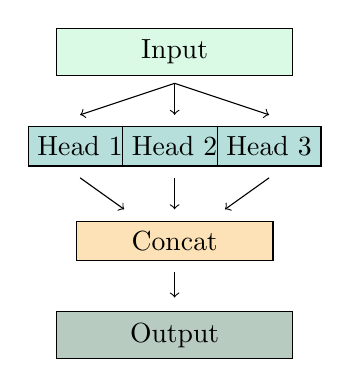
\begin{tikzpicture}[scale=0.8]
    % Draw multi-head attention diagram
    \node[draw, fill=LightGreen!30, minimum width=3cm, minimum height=0.6cm] at (0,4) {Input};

    % Three attention heads
    \node[draw, fill=Teal!30, minimum width=0.8cm, minimum height=0.5cm] at (-1.5,2.5) {Head 1};
    \node[draw, fill=Teal!30, minimum width=0.8cm, minimum height=0.5cm] at (0,2.5) {Head 2};
    \node[draw, fill=Teal!30, minimum width=0.8cm, minimum height=0.5cm] at (1.5,2.5) {Head 3};

    % Concatenation
    \node[draw, fill=Amber!30, minimum width=2.5cm, minimum height=0.5cm] at (0,1) {Concat};

    % Output
    \node[draw, fill=ForestGreen!30, minimum width=3cm, minimum height=0.6cm] at (0,-0.5) {Output};

    % Arrows
    \draw[->] (0,3.5) -- (-1.5,3);
    \draw[->] (0,3.5) -- (0,3);
    \draw[->] (0,3.5) -- (1.5,3);
    \draw[->] (-1.5,2) -- (-0.8,1.5);
    \draw[->] (0,2) -- (0,1.5);
    \draw[->] (1.5,2) -- (0.8,1.5);
    \draw[->] (0,0.5) -- (0,0.1);
\end{tikzpicture}

\vspace{3mm}
\begin{alertblock}{Future Directions}
\begin{enumerate}
    \item \natureemph{Cross-lingual} models
    \item \natureemph{Multimodal} seq2seq
    \item \natureemph{Few-shot} learning
\end{enumerate}
\end{alertblock}
\end{column}
\end{columns}
\end{frame}

% Summary
\section{Summary}
\begin{frame}{Key Takeaways}
\begin{columns}[T]
\begin{column}{0.48\textwidth}
\begin{block}{What We Learned}
\begin{enumerate}
    \item \natureconcept{Encoder-Decoder} architecture
    \item \naturehighlight{Attention mechanism} importance
    \item \natureemph{Beam search} for decoding
    \item Training dynamics and optimization
    \item Evolution to Transformers
\end{enumerate}
\end{block}

\begin{exampleblock}{Practical Applications}
\begin{itemize}
    \item Machine Translation
    \item Text Summarization
    \item Dialog Systems
    \item Code Generation
    \item Image Captioning
\end{itemize}
\end{exampleblock}
\end{column}

\begin{column}{0.48\textwidth}
\begin{alertblock}{Next Steps}
\begin{itemize}
    \item Week 5: \naturehighlight{Transformers}
    \item Week 6: \natureemph{Pre-trained Models}
    \item Week 7: \natureconcept{Advanced Architectures}
\end{itemize}
\end{alertblock}

\vspace{5mm}
\begin{center}
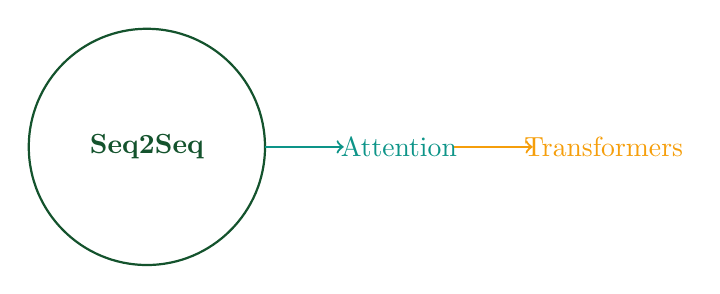
\begin{tikzpicture}
    % Summary visualization
    \draw[thick, ForestGreen] (0,0) circle (1.5cm);
    \node at (0,0) {\textcolor{ForestGreen}{\textbf{Seq2Seq}}};
    \draw[thick, Teal, ->] (1.5,0) -- (2.5,0);
    \node at (3.2,0) {\textcolor{Teal}{Attention}};
    \draw[thick, Amber, ->] (3.9,0) -- (4.9,0);
    \node at (5.8,0) {\textcolor{Amber}{Transformers}};
\end{tikzpicture}
\end{center}

\vspace{5mm}
\begin{center}
\Large\natureconcept{Thank You!}
\end{center}
\end{column}
\end{columns}
\end{frame}

\end{document}